\documentclass[11pt]{article}
\usepackage[utf8]{inputenc}
\usepackage[toc,page]{appendix}
\usepackage{microtype}
\usepackage{fullpage}
\usepackage{multirow}

\usepackage{minted}
\setminted[]{linenos, numbersep=5pt, frame=lines}

\usepackage{parskip}
\setlength{\parindent}{0em}
\setlength{\parskip}{1em}


\usepackage[affil-it]{authblk}
\usepackage{amsfonts, amssymb, amsmath}

\usepackage{wrapfig}
\usepackage{graphicx}
\graphicspath{ {./images/} }

\usepackage{float}

\usepackage[backend=biber]{biblatex}
\addbibresource{sources.bib}
% Use the followign Command to validate *.bib file: biber --tool --validate-datamodel qualifying_exam_paper.bib

\title{Improving Emotion Detection through Real-Time Translation of Text to ML Models Trained in Different Languages}

\author{Richard Hoehn%
	\thanks{Electronic address: \texttt{rhoehn@mtmail.mtsu.edu}; corresponding author}}
\affil{Middle Tennessee State University}

\author{Dr. Jaishree Ranganathan%
	\thanks{Electronic address: \texttt{jaishree.ranganathan@mtsu.edu}}}
\affil{Middle Tennessee State University}


\begin{document}

\maketitle

\begin{abstract}
This Qualifying Exam\footnote{PhD students of MTSU Computational and Data  Science program are required to complete a Qualifying Exam in their first year in the program.} research paper investigates the potential of improving Emotion Detection (ED) through real-time translation of text to multiple Machine Learning (ML) models trained in different languages. The research tries to address the challenges posed by the lack of comprehensive labeled datasets and language fragmentation in ED analysis.

By extending an original language dataset with a translated dataset from another language and utilizing parallel processing with PySpark, this research project aims to achieve higher prediction rates in ED. The results presented both orally to the MTSU's Computational Data \& Science Committee and within this paper demonstrate the effectiveness of such an approach and how the real-time translation technique can enhance emotion detection capabilities.
\end{abstract}
\clearpage

\tableofcontents
\clearpage

\section{Introduction}
\subsection{Background on Human Emotion Theoretical Framework}

\begin{wrapfigure}{r}{0.4\textwidth} %this figure will be at the right
    \centering
    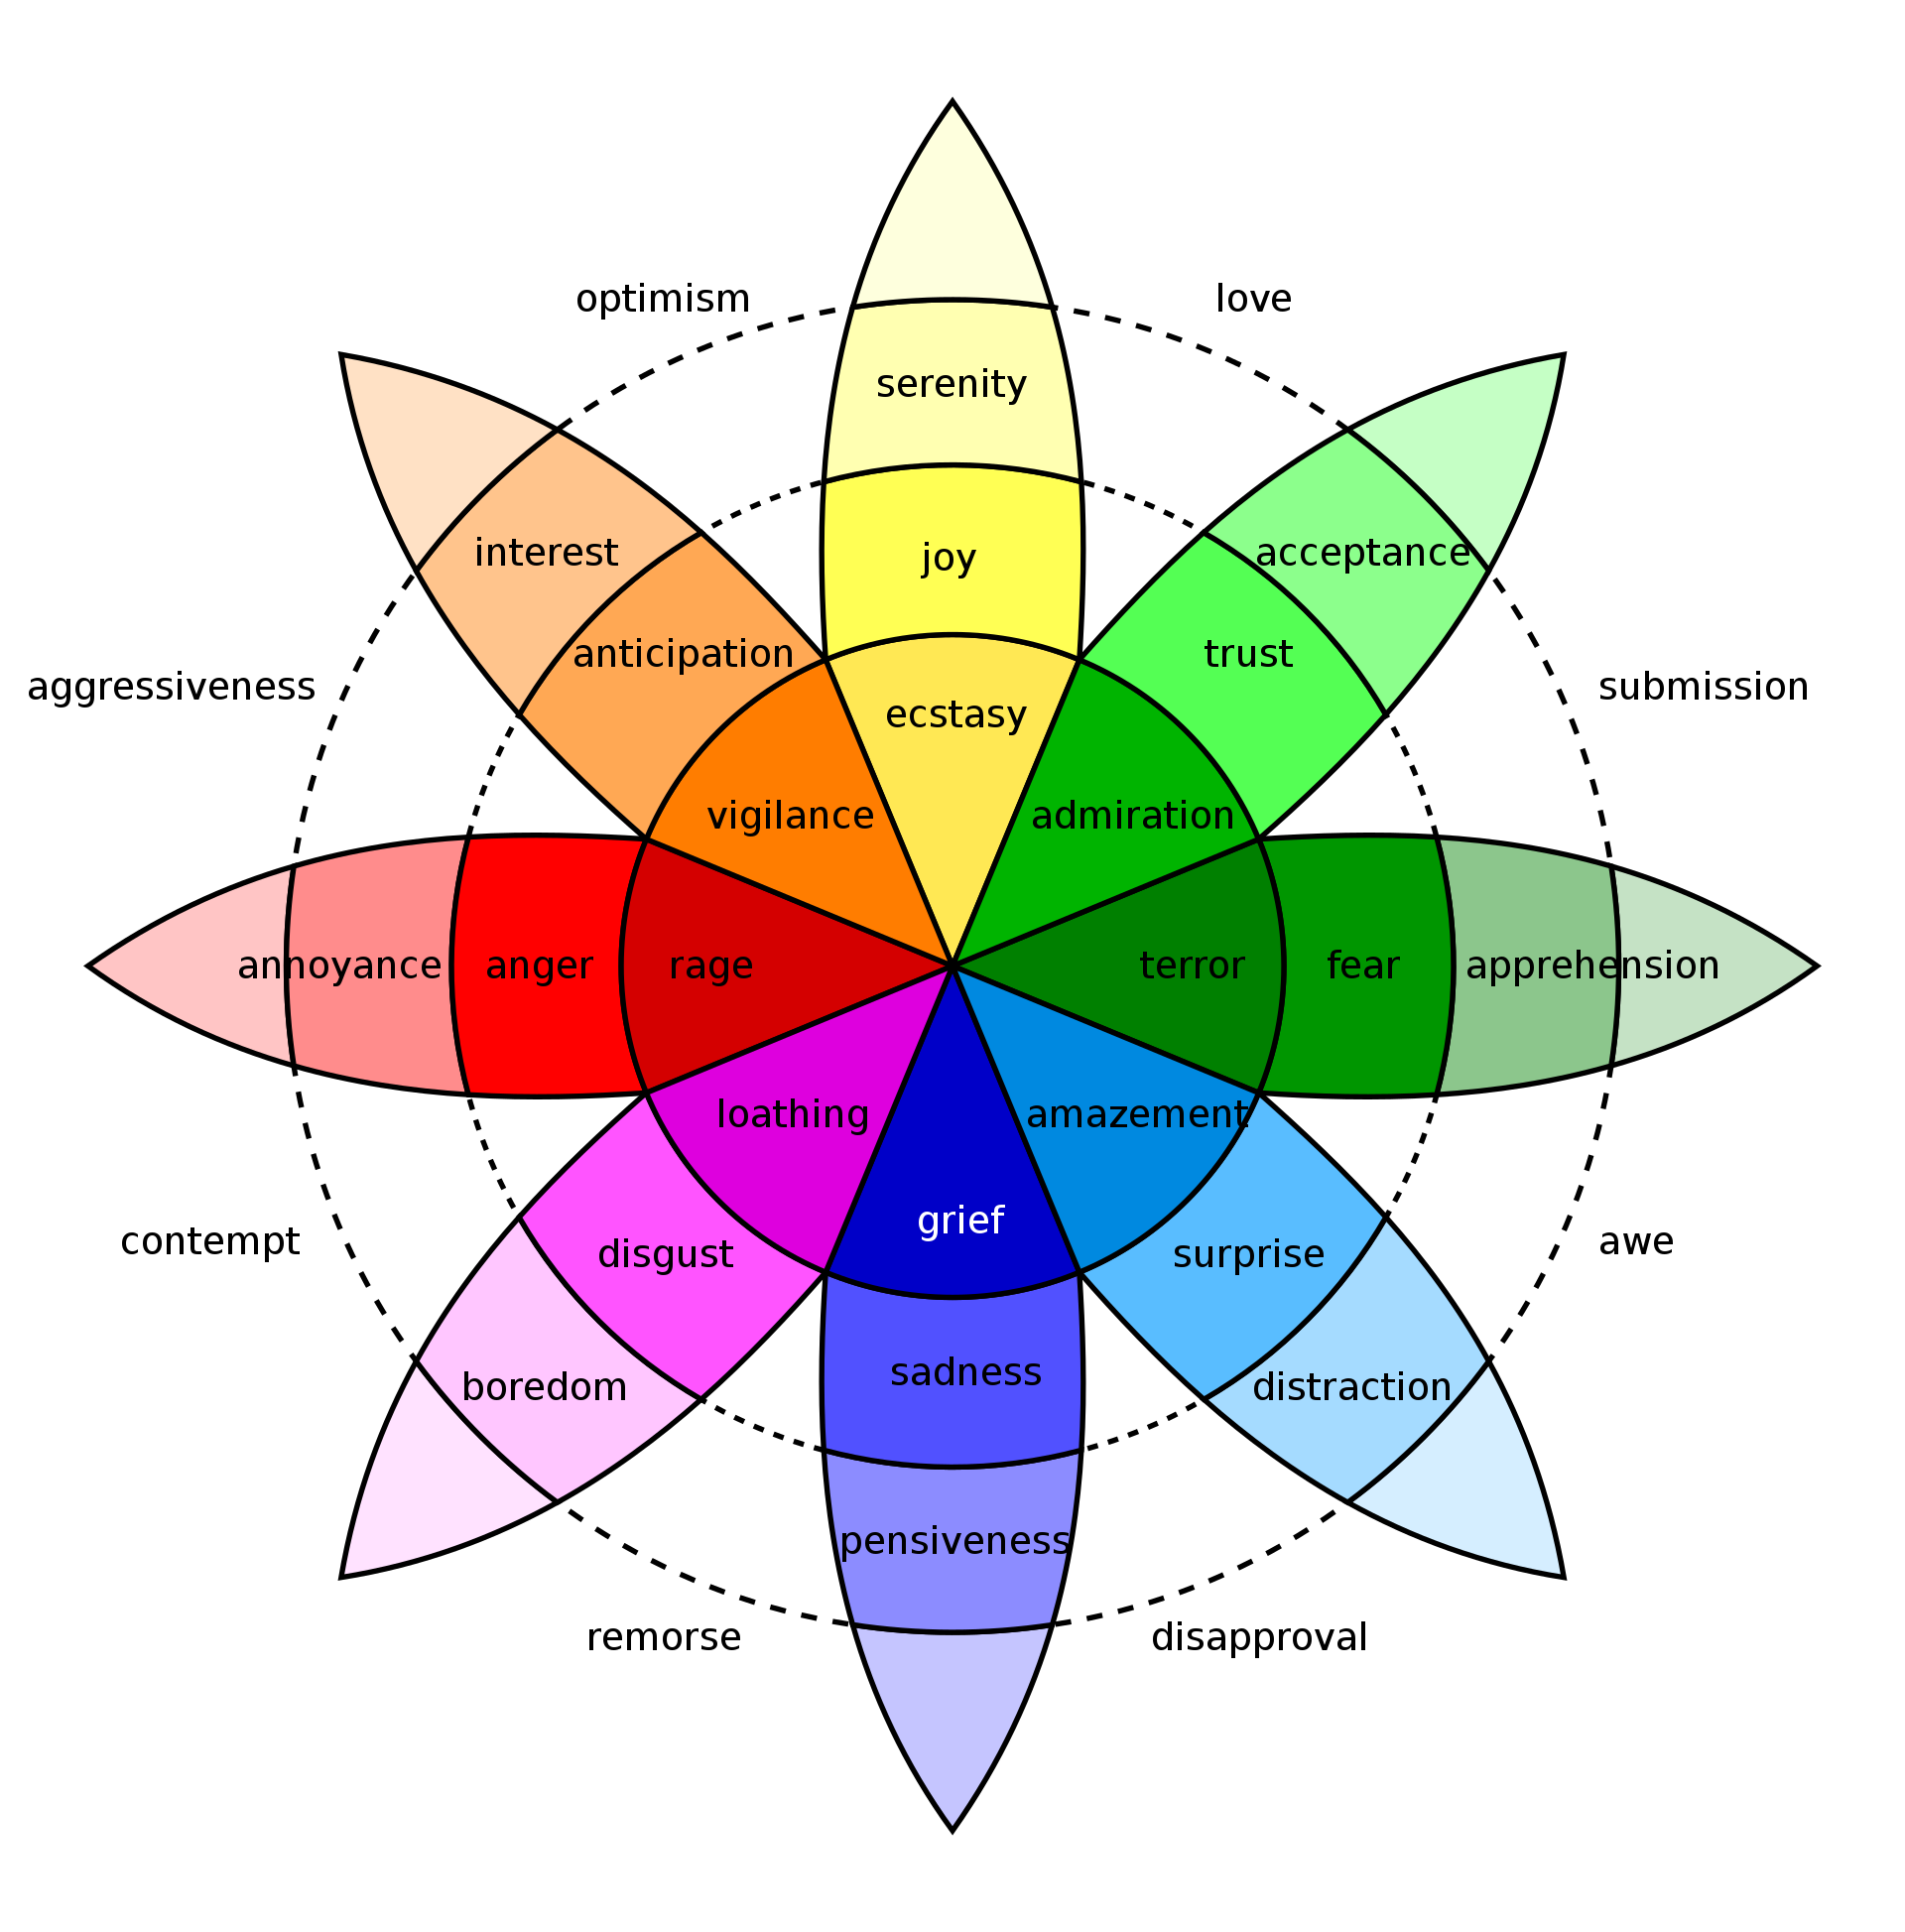
\includegraphics[width=0.35\textwidth]{Plutchik-Wheel}
    \caption{Plutchik Wheel of Emotions}
    \label{fig:plutchik-wheel}
\end{wrapfigure}

The concept of the eight main emotions can vary depending on the theoretical framework or model being considered. One well-known model is the Plutchik's Wheel of Emotions figure \ref{fig:plutchik-wheel}, which proposes eight primary emotions and their contrasting pairs. Here are the eight primary emotions according to the Plutchik's Wheel of Emotions \cite{Tromp}:

\begin{itemize}
\item Joy (Fun): A feeling of happiness, contentment, or delight.
\item Sadness: A state of unhappiness, sorrow, or grief.
\item Anger: An intense emotional response associated with feelings of displeasure, frustration, or hostility.
\item Worry: An emotional response triggered by perceived threats or danger, often associated with anxiety or terror.
\item Surprise: A sudden and unexpected reaction to something unusual or startling.
\item Disgust (Hate): A strong aversion or revulsion towards something unpleasant, offensive, or repulsive.
\item Trust: A sense of reliance, confidence, or faith in someone or something.
\item Anticipation: A feeling of excited expectation or eagerness towards future events.
\end{itemize}
It's important to note that emotions are complex and multifaceted, and different models may propose alternative categorizations or variations in the number of primary emotions. However for the scope of this research project the most common 8 emotions are used as described above. Both the English and German datasets being used in this research matched to the 8 listed above. Details on the linkage of the two datasets is described in the next section with an emphasis on the Table \ref{table:dataset_labels} detailed linkage.

\subsection{Background and significance of Emotion Detection (ED) analysis in Machine Learning models}
Emotion Detection (ED) analysis in Machine Learning (ML) models has gained significant attention due to its potential applications in various fields, including customer sentiment analysis, stance detection in regard to a specific targets such as news and voting\cite{mascarell-etal-2021-stance}, mental health monitoring\cite{Colonnello}, and human-computer interactions to just name a few.

By accurately identifying and understanding emotions from text data, ML models can assist in improving user experiences, decision-making processes, and overall human-machine interactions in a positive manner\cite{Colonnello, mascarell-etal-2021-stance}. With the goal in mind of improving ML models this research paper came to be.

\begin{quote}
    I usually know almost exactly how I feel. The problem is, I just can’t tell anyone.
    \flushright -- Meg Cabot
\end{quote}

Due to the before mentioned wide scope of uses for ED this field of research and the work to advance it provides significance and importance in enabling machines to comprehend and respond appropriately to human emotions. This in turn contributes to the advancement of artificial intelligence, natural language processing and in many cases the utilization of text-to-speech applications most all of us in today's society use and rely on.

\subsection{ED challenges, including lack of comprehensive labeled datasets and language fragmentation}
ED is growing field, however unlike Sentiment Analysis (SA) the availability of large datasets for training purposes of ML models is much smaller. The primary reason of the lack of data stems from the emotion detection requiring primarily supervised learning dataset, which require time and effort to procure, and mostly created by humans. To compound on the issue of the lack of data; the many datasets that are available are in multiple languages.

\subsection{Motivation for the research project focusing on extending ED datasets through translation and evaluating the impact on prediction rates}

This paper is significant because an entire industry of automated purported emotion reading (Text, Image, Video, and Sound) technologies is quickly emerging \cite{ACLU-ED-Data, ACLU-THE-DAWN-OF-ROBOT-SURVEILLANCE}. The market for emotion recognition software is forecast to reach at least \$3.8 billion by 2025 \cite{ACLU-ED-Data, ACLU-THE-DAWN-OF-ROBOT-SURVEILLANCE}. And since ED is already being incorporated into products for purposes such as marketing, robotics, driver safety, and a multiple of others, it is fitting to work on research to solve issues.

With the before mentioned issues regarding the quantity/lack and fragmentation of the ED datasets this research was motivated by finding a way to combine different language datasets into a single set for training processes to improve the predictability of ED. The hope is that by use of translation that the predictability of ED can be improved by use of real- real-time language conversion and processing.

\subsection{Objectives \& Scope of the Research}
The project is comprised of three main points / goals which are listed in following sub-sections with details in each point as follows:

\subsubsection{Data Collection / Translation / ML Model Training}

\begin{wrapfigure}{R}{0.4\textwidth} %this figure will be at the right
    \centering
    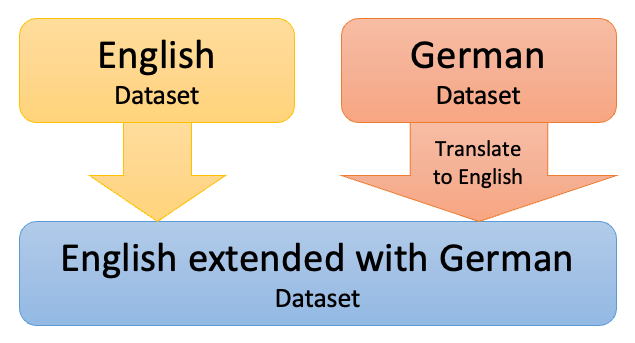
\includegraphics[width=0.35\textwidth]{Dataset-Extension}
    \caption{Example of English dataset extension by translating from German.}
    \label{fig:dataset-extension}
\end{wrapfigure}

The procurement of two ED datasets is needed. The first will be in English and the second in German. Each dataset will be translated into the other’s language for extending purposes. As an example Figure \ref{fig:dataset-extension} depicts the original English dataset will be extended by the translated German dataset.

The reason for selecting German was based on the author\footnote{Richard Hoehn} being fluent in English and German and hence being able to easily traverse the two languages while working on the code for dataset translations and formatting.

Once the two datasets have been translated, we now extend the original language dataset with the translated one.By this approach we are in essence extending the original datasets to create a larger one wiht the foreign language data. With both extended datasets we can now train our ML models for English and German.

\subsubsection{PySpark Application Development for Translation \& Prediction}
A program will be built in Jupiter Notebooks that uses translations APIs to convert an English sentence to German and the same if a German sentence is fed to English. Both sentences are then processed in real-time on both the English and German models for the Emotion Detection and will be compared to each other's output. The average of the prediction will be used for final prediction of the supplied sentence and the emotion that was detected.

In order for such to be processed in real-time, the Jupyter Notebook will start a PySpark session that is accessed via the local server running that accepts RESTful API calls with details of the server in Appendix \ref{appendix:code-api-server}.

\subsubsection{Written \& Oral Presentation of Research Finding}
In conclusion of the project a research paper and oral presentation is required to pass MTSU Computation Science PhD Qualifying Exam. Such paper is being presented with this paper and the oral presentation will be in Microsoft Power Point format.

The listing the datasets used, code for the application, and details of the research project process in this research paper is openly available and hosted on a GitHub repository, allowing for easy access, reproducible, and collaborative engagement with the research findings. The repository is open and available under: \texttt{https://github.com/richardhoehn/mtsu.coms.qualifying-exam}\cite{Hoehn_Improving_Emotion_Detection_2023}

\section{Literature Review}

\subsection{Emotion Detection Importance, Data Limitations, Diverse Populations}
Emotion Detection (ED) holds significant importance in various domains, including psychology, social sciences, and human-computer interaction. It enables the analysis of human emotions at scale, providing valuable insights into individual and collective emotional states. However, the field faces limitations due to the scarcity of comprehensive labeled datasets. The lack of diverse and large-scale data hinders the development and training of accurate ED models, limiting their effectiveness and general ability across different contexts and populations.

In recent research, efforts have been made to address these limitations by exploring new techniques for emotion detection. For instance, a study by Shalini Kapoor, Tarun Kumar \cite{KAPOOR2023120882} proposes analyzing the entire spectrum of the language source to predict emotional changes. 

Overcoming the scarcity of labeled datasets and embracing innovative approaches like the before mentioned study by Shalini Kapoor, Tarun Kumar \cite{KAPOOR2023120882} and their analysis can contribute to the advancement of ED research. Such advancements hold the potential to enhance the accuracy and applicability of emotion detection models, enabling a deeper understanding of human emotions and more effective responses in various domains.

Emotions can differ across age groups, genders, cultures, and languages. Including data from diverse populations helps in developing inclusive and culturally sensitive ED models. It ensures that the models are not biased towards specific groups and can accurately detect emotions in a wide range of individuals.

\subsection{Challenges by the lack of Labeled Datasets and the Fragmentation caused by Different Languages}
Unlike images language operate very differently, therefore the lack of labeled datasets poses a significant challenge in text-based Emotion Detection (ED) analysis as it limits the availability of reliable training data for ML models. This scarcity hampers the model's ability to learn and generalize emotions effectively. Additionally, the fragmentation caused by different languages further exacerbates the issue, as it reduces the size and diversity of data available for training, resulting in limited cross-lingual generalization and potentially biased models. Overcoming these challenges is crucial for advancing ED research and improving the accuracy and applicability of emotion detection models across various languages and cultures.

\section{Methodology}

\subsection{Data procurement process, including obtaining ED datasets in English and German}
The data procurement was relatively straight forward and in essence entailed using Google search terms for the Emotion Detection in English and German. Some of the main German data was obtained from the dataset built by ETH's Emotion and Stance Detection for German Text \cite{mascarell-etal-2021-stance} which also hosts a good website with their finds \footnote{https://mtc.ethz.ch/research/natural-language-processing/emotion-stance.html}. The English dataset was downloaded from Kaggle \footnote{https://www.kaggle.com/datasets/pashupatigupta/emotion-detection-from-text} based on Tweets collected in 2021. The English dataset contains over 38,000 tweets and their corresponding emotion labeled. Similarly the German contains over 12,000 sentences and their respective emotions associated.

An important part of the process is to make sure we match the English emotions to those of the German language emotions. Since the tow languages are dissimilar we opted to match exact emotions to each other that can be seen in Table \ref{table:dataset_labels} below.

\begin{table}[h!]
\centering
\begin{tabular}{ | c c | c c | c | }
    \hline
    \multicolumn{5}{|c|}{Emotion Datasets Labels} \\
    
    \hline
    \multicolumn{2}{|c|}{English} & \multicolumn{2}{|c|}{German} & \multirow{2}{*}{Used} \\
    Name & Count & Name & Count \\
    \hline
    Boredom    &  179 & ---           & --- & NO  \\
    Love       & 3842 & Vertrauen     & 316 & YES \\
    Relief     & 1526 & ---           & --- & NO  \\ 
    Fun        & 1776 & ---           & --- & NO  \\
    Hate       & 1323 & Ekel          &  29 & YES \\
    Neutral    & 8638 & Unklar        & 314 & YES \\
    Anger      &  110 & Ärger         & 226 & YES \\
    Happiness  & 5209 & Freude        & 140 & YES \\
    Surprise   & 2187 & Überraschung  & 369 & YES \\
    Sadness    & 5165 & Traurigkeit   & 184 & YES \\
    Worry      & 8459 & Angst         & 154 & YES \\
    Enthusiasm &  759 & Antizipation  & 774 & YES \\
    Empty      &  827 & ---           & --- & NO  \\
    \hline
\end{tabular}
\caption{Dataset of English \& German and their respective label counts.}
\label{table:dataset_labels}
\end{table}

Details on how we formatted the the two (English and German) datasets to each other can be viewed in the Appendix \ref{appendix:dataset_english} and \ref{appendix:dataset_german}

\subsection{Development of a translation application for converting different languages into English and vice versa}
Translation of the emotion datasets was performed with Google Translator based on the Medium article\cite{Nidhaloff_how_to_translate_text_with_python} in which the author describes option fro simple API translations. As an example the following is a brief introduction to Google Translator's API:

\begin{quote}
\begin{minted}[fontsize=\small]{python}
# Using Deep Translator to leveage Google Translate
# Link: https://cloud.google.com/translate/docs/reference/libraries/v2/python
from deep_translator import GoogleTranslator

sentence = 'Chocolate milk is so much better through a straw.'

translated = GoogleTranslator(source='auto', target='de').translate(sentence)
print(translated) # Schokoladenmilch schmeckt durch einen Strohhalm viel besser.

translated_back = GoogleTranslator(source='auto', target='en').translate(translated)
print(translated_back) # Chocolate milk tastes much better through a straw.
\end{minted}
\end{quote}


\subsection{Building and training multiple ML models using the extended datasets and parallel processing approach with PySpark}
\ldots

\subsection{Evaluation Metrics and methodologies for measuring the performance of the ML models}
The evaluation of ML models trained on text datasets is a critical step in assessing their performance and reliability. Our research project is no different and the following assumptions are used to determine the effectiveness of the methodology of extending our datasets:
\begin{itemize}
\item \textbf{Accuracy:} Accuracy measures the overall correctness of the emotion predictions made by the model. It is calculated as the ratio of correctly classified instances to the total number of instances in the dataset. However, accuracy may not provide a complete picture, especially if the dataset is imbalanced.
\item \textbf{Precision, Recall, and F1 Score:} Precision represents the proportion of correctly predicted emotions among all instances predicted as a specific emotion. Recall measures the proportion of correctly predicted emotions among all instances that truly belong to a specific emotion. F1 score combines precision and recall into a single metric, providing a balanced evaluation.
\item \textbf{Cross-Validation:} Cross-validation techniques, such as k-fold or stratified cross-validation, divide the dataset into multiple subsets for training and testing. This helps evaluate the model's performance across different data samples, mitigating over-fitting and providing a more robust estimation of its generalization ability.
\item \textbf{Error Analysis:} Performing error analysis on the model's predictions helps identify specific patterns or instances where the model might struggle or make frequent mistakes. This analysis can guide improvements and provide insights for future model development.
\end{itemize}

When evaluating such models, several factors come into play. First and foremost, the choice of appropriate evaluation metrics is crucial, depending on the specific task at hand, such as text classification, sentiment analysis, or named entity recognition. Metrics like accuracy, precision, recall, F1 score, or area under the receiver operating characteristic curve (AUC-ROC) are commonly used to measure the models' performance.



\section{Results and Analysis}

\subsection{Presentation of the prediction results obtained from the extended datasets}

\ldots

\subsection{Comparison of Prediction Result of the Original and Extended Language (translated) Datasets}
\ldots

\subsection{Analysis of the impact of Extending Datasets by Translation and Performance of the Combination of ML models}
\ldots

\subsection{Discussion of the findings and their implications for improving Emotion Detection}
\ldots

\section{Demonstration and Application}

\subsection{Description of the developed translation application for real-time text translation}
Details of the entire application can be found on the github repository \cite{Hoehn_Improving_Emotion_Detection_2023}.

\subsection{Showcase of the application's functionality and its integration with the Emotion Detection process}
\ldots

\subsection{Demonstration of the real-time processing of translated text and emotion detection using the ML models}
\ldots

\subsection{GIT Repository Details}
The listing the datasets used, code for the application, and details of the research project process in this research paper is openly available and hosted on a GitHub repository, allowing for easy access, reproducible, and collaborative engagement with the research findings. The repository is open and available under: \texttt{https://github.com/richardhoehn/mtsu.coms.qualifying-exam}\cite{Hoehn_Improving_Emotion_Detection_2023}
\clearpage


\addcontentsline{toc}{section}{References}
\printbibliography
\clearpage


\addcontentsline{toc}{section}{List of Figures}
\listoffigures
\clearpage

% Appendix Details
\appendix
\section{Appendix -- Dataset Details}
The following details in this appendix are for clarification purposes.
All examples in this appendix are created via PySpark using dataframes.

\subsection{Using PySpark to Load Data}
All example code was created using Jupyter Notebooks creating a PySpark session. The details of setting up such session are below in the code example. All subsequent details are derived from the \texttt{sc}\footnote{sc = Spark Session}.
\begin{minted}[fontsize=\small]{python}
# General Imports
import glob
import shutil

# Setup Spark Session
from pyspark.sql import SparkSession

# Get Spark Functions Needed
from pyspark.sql.functions import col, udf, split, explode

# Get Datatypes needed for DataFrame manipulation
from pyspark.sql.types import IntegerType, StringType

# Setup Spark Session
sc = SparkSession \
        .builder \
        .master("local[*]") \
        .appName("data_clean_up") \
        .getOrCreate()

# Print Spark Version being run
print("Spark V: ", sc.version)
\end{minted}
\clearpage


\subsection{Details on English Dataset}
\label{appendix:dataset_english}
The English dataset is based on tweets\footnote{Tweets from Twitter} that are saved as a \texttt{csv}\footnote{csv = Comma Separated Values} file. The following code was use to filter and process the file for use in this project.
\begin{minted}[fontsize=\small]{python}
# *********************************
# *** English Data Preparations ***
# *********************************

# Load English CSV File into a Dataframe
df_english = sc.read.csv("data/english.csv", header=True, inferSchema=True)
print(f'Count (raw): {df_english.count()}')

# Print Columns
print(f'English Source Columns: {df_english.columns}\n')

# Filter only lavbels that we mathc with the German counter parts
filter_values = ["love", "hate", "neutral", "anger", "happiness", "surprise", "sadness", "worry", "enthusiasm"]
df_english_filtered = df_english.filter(col("sentiment").isin(filter_values))

# Remove unnecessary column
df_english_filtered = df_english_filtered.drop("tweet_id")

# Rename Columns
df_english_filtered = df_english_filtered.withColumnRenamed("sentiment", "emotion_en")
df_english_filtered = df_english_filtered.withColumnRenamed("content", "sentence_en")

# Make sure the column order to the same for both german and english csv files
df_english_filtered = df_english_filtered.select('sentence_en', 'emotion_en')

print(f'Count (filtered): {df_english_filtered.count()}')

# Group By for Details & Count
df_english_grouped = df_english_filtered.groupBy('emotion_en').count()

# Show Groupings and Respetive Counts
print('\nGrouped & Count by "emotion"')
df_english_grouped.show(truncate=0)


# Save Dataframe to CSV
directory_path = 'data/spark_data_parts'
df_english_filtered.coalesce(1).write.csv(directory_path, header=True, mode="overwrite")

file_pattern = 'part-00000*.csv'
file_path = glob.glob(directory_path + '/' + file_pattern)[0]

shutil.move(file_path, './data/data_en.csv')

Count (raw): 40000
English Source Columns: ['tweet_id', 'sentiment', 'content']

Count (filtered): 35692

Grouped & Count by "emotion"
+----------+-----+
|emotion_en|count|
+----------+-----+
|love      |3842 |
|hate      |1323 |
|neutral   |8638 |
|anger     |110  |
|happiness |5209 |
|surprise  |2187 |
|sadness   |5165 |
|worry     |8459 |
|enthusiasm|759  |
+----------+-----+
\end{minted}
\clearpage

\subsection{Details on German Dataset}
\label{appendix:dataset_german}
The German dataset was downloaded from the ETH's\footnote{ETH (German: Eidgenössische Technische Hochschule) or Swiss Federal Institute of Technology} servers via "link" as a \texttt{JSON} file. Since the the file was \texttt{JSON} we will need to filter and explode the file based on teh emotions that are attached to it.
\begin{minted}[fontsize=\small]{python}
# ********************************
# *** German Data Preparations ***
# ********************************

# Load German JSON File into a Dataframe
df_german = sc.read.json("data/german.json")
print(f'Count (raw): {df_german.count()}')

# Print Columns
print(f'German Source Columns: {df_german.columns}\n')


# We Need to "split" the "artice_emotion" column since the ETH team listed
# multiple emotions in one column
# In order to "explode" the column to it's distinct rows
df_german_exploded = df_german.select('*', explode('article_emotion').alias('emotion_de'))

# Rename Column
df_german_exploded = df_german_exploded.withColumnRenamed("title", "sentence_de")

# Remove unnecessary column
df_german_exploded = df_german_exploded.drop("article_id")
df_german_exploded = df_german_exploded.drop("article_stance")
df_german_exploded = df_german_exploded.drop("paragraphs")
df_german_exploded = df_german_exploded.drop("source")
df_german_exploded = df_german_exploded.drop("article_emotion")
df_german_exploded = df_german_exploded.drop("snippet")

# Make sure the column order to the same for both german and english csv files
df_german_exploded = df_german_exploded.select('sentence_de', 'emotion_de')

print(f'Count (filtered): {df_german_exploded.count()}')

# Group By for Details & Count
df_german_grouped = df_german_exploded.groupBy('emotion_de').count()

# Show Groupings and Respetive Counts
print('\nGrouped & Count by "emotion"')
df_german_grouped.show(truncate=0)


# Save Dataframe to CSV
directory_path = 'data/spark_data_parts'
df_german_exploded.coalesce(1).write.csv(directory_path, header=True, mode="overwrite")

file_pattern = 'part-00000*.csv'
file_path = glob.glob(directory_path + '/' + file_pattern)[0]

shutil.move(file_path, './data/data_de.csv')

Count (raw): 1970
German Source Columns: ['article_emotion', 'article_id', 'article_stance', 'paragraphs', 'snippet', 'source', 'title']

Count (filtered): 2568

Grouped & Count by "emotion"
+------------+-----+
|emotion_de  |count|
+------------+-----+
|Vertrauen   |316  |
|Freude      |140  |
|Ärger       |226  |
|Überraschung|369  |
|Traurigkeit |184  |
|Antizipation|774  |
|Unklar      |314  |
|Angst       |154  |
|Ekel        |29   |
|Keine       |62   |
+------------+-----+
\end{minted}
\clearpage


\subsection{Details on Extending \& Translation}
\label{appendix:dataset_translation}
Details on translation and extending the datasets.
\begin{minted}[fontsize=\small]{python}
# **************************************
# *** English <-> German Emotion Key ***
# **************************************


from pyspark.sql.functions import col, udf, split, explode, lit
from pyspark.sql.types import IntegerType, StringType, StructType, StructField, StringType

# Emotion Dictionary English <-> German
# This key/value setup was previsoulsy created for linking purposes
emotion_key = {
    "boredom"    : "---",
    "love"       : "Vertrauen",
    "relief"     : "---",
    "fun"        : "---",
    "hate"       : "Ekel",
    "neutral"    : "Unklar",
    "anger"      : "Ärger",
    "happiness"  : "Freude",
    "surprise"   : "Überraschung", 
    "sadness"    : "Traurigkeit", 
    "worry"      : "Angst",
    "enthusiasm" : "Antizipation", 
    "empty "     : "---",
    "---"        : "Keine",
}

# Create the schema for the DataFrame
schema = StructType([
    StructField("emotion_en", StringType(), nullable=False),
    StructField("emotion_de", StringType(), nullable=False)
])

# Convert the dictionary to a list of tuples
data = [(key, value) for key, value in emotion_key.items()]

# Create the PySaprk DataFrame
df_emotion_key = sc.createDataFrame(data, schema)

df_emotion_key.show()

# Extend the English and German onto the datasets
df_german_exploded = df_german_exploded.join(df_emotion_key, on="emotion_de", how="left")
df_english_filtered = df_english_filtered.join(df_emotion_key, on="emotion_en", how="left")

# New sentence column
df_german_exploded = df_german_exploded.withColumn("sentence_en", lit(None))
df_english_filtered = df_english_filtered.withColumn("sentence_de", lit(None))

df_german_exploded.show()
df_english_filtered.show()


# Using Deep Translator to proxy to Google Translate
from deep_translator import GoogleTranslator


# Define Tranlation Functions
def translate_en_to_de(row):
    translated = GoogleTranslator(source='en', target='de').translate(row["sentence_en"])
    row["sentence_de"] = translated

def translate_de_to_en(row):
    translated = GoogleTranslator(source='de', target='en').translate(row["sentence_en"])
    row["sentence_en"] = translated
    

df_german_exploded.foreach(translate_de_to_en)  

+----------+------------+
|emotion_en|  emotion_de|
+----------+------------+
|   boredom|         ---|
|      love|   Vertrauen|
|    relief|         ---|
|       fun|         ---|
|      hate|        Ekel|
|   neutral|      Unklar|
|     anger|       Ärger|
| happiness|      Freude|
|  surprise|Überraschung|
|   sadness| Traurigkeit|
|     worry|       Angst|
|enthusiasm|Antizipation|
|    empty |         ---|
|       ---|       Keine|
+----------+------------+

+------------+--------------------+----------+----------+-----------+----------+
|  emotion_de|         sentence_de|emotion_en|emotion_en|sentence_en|emotion_en|
+------------+--------------------+----------+----------+-----------+----------+
|   Vertrauen|Adoptiert zu sein...|      love|      love|       null|      love|
|      Freude|Österreichs Verfa...| happiness| happiness|       null| happiness|
|      Freude|Visana gewinnt er...| happiness| happiness|       null| happiness|
\end{minted}
\clearpage
 % Note: SubSection headers are handled within the *.tex file 
\section{Appendix -- Application \& Code Details}
Hello World - Application \& Code Details
\subsection{Application}
\label{appendix:code_application}
Hello World - Application
\clearpage

\subsection{Code Details}
Hello World - Code Details

\subsection{RESTful API Server}
\label{appendix:code-api-server}
The RESTful\footnote{RESTful API is an interface that two computer systems use to exchange information securely over the internet.} API Server will be a simple Python Flask server listening on port \texttt{8080} on the local machine.


\clearpage
 % Note: SubSection headers are handled within the *.tex file 

\end{document}



